\documentclass{article}
\usepackage{tikz}
\usetikzlibrary{positioning,calc}
\begin{document}
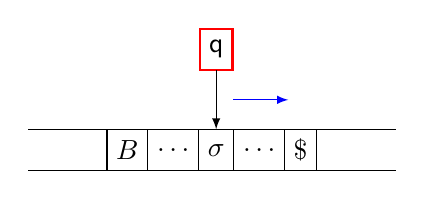
\begin{tikzpicture}[every node/.style={block},
        block/.style={minimum height=1.5em,outer sep=0pt,draw,rectangle,node distance=0pt}]
   \node (A) {$\sigma$};
   \node (B) [left=of A] {$\ldots$};
   \node (C) [left=of B] {$B$};
   \node (D) [right=of A] {$\ldots$};
   \node (E) [right=of D] {$\$ $};
   \node (F) [above = 0.75cm of A,draw=red,thick] {\textsf q};
   \draw[-latex] (F) -- (A);
   \draw[-latex,blue] ($(F.east)!0.5!(A.east)$) -- ++(7mm,0);
   \draw (C.north west) -- ++(-1cm,0) (C.south west) -- ++ (-1cm,0) 
                 (E.north east) -- ++(1cm,0) (E.south east) -- ++ (1cm,0);
\end{tikzpicture}
\end{document}